\documentclass[11pt,a4paper]{article}

\usepackage{graphicx}
\usepackage{xcolor}
\usepackage{geometry}
\usepackage{amsmath}
\usepackage{amssymb}
\usepackage{booktabs}
\usepackage{tabularx}
\usepackage{adjustbox}
\usepackage{enumitem}
\usepackage{microtype}
\usepackage[numbers,super,sort&compress]{natbib}

\geometry{a4paper, top=2.4cm, bottom=2.4cm, left=2.2cm, right=2.2cm}

\usepackage[colorlinks=true, linkcolor=blue!60!black, citecolor=blue!60!black,
            urlcolor=blue!60!black, bookmarks=true, bookmarksnumbered=true,
            unicode=true]{hyperref}

\widowpenalty=10000
\clubpenalty=10000
\setlength{\parskip}{0pt}

\newcommand{\deepens}{\textsc{DeepEns}}
\newcommand{\snapshot}{\textsc{Snapshot}}
\newcommand{\swa}{\textsc{SWA}}
\newcommand{\single}{\textsc{Single}}

\hypersetup{
  pdftitle={Budget-split deep ensembles outperform snapshot ensembles and weight averaging for calibrated uncertainty},
  pdfauthor={Z.ai},
  pdfsubject={Budget-matched comparison of ensemble strategies for predictive uncertainty},
  pdfkeywords={deep ensembles, snapshot ensembles, stochastic weight averaging, calibration, uncertainty quantification, budget-matched evaluation}
}

\begin{document}

% ─────────────────────────────── title block ───────────────────────────────
\begin{center}
{\LARGE\bfseries Budget-split deep ensembles outperform snapshot ensembles\\[2pt] and weight averaging for calibrated uncertainty\par}
\vspace{10pt}
{\small Prepared with the Qinyan Nature Skills research workflow; authorship and affiliations pending author confirmation.\par}
\vspace{4pt}
{\small Preprint, 22 September 2026. Ten seeded replications. Code and source data available.\par}
\end{center}
\vspace{6pt}

\noindent\rule{\textwidth}{0.4pt}
\begin{center}
\begin{minipage}{0.93\textwidth}
\small
\textbf{Abstract} \quad Well-calibrated predictive uncertainty is a requirement for deploying classifiers in safety-relevant settings, yet practitioners usually face a fixed training-compute budget rather than the unconstrained budgets assumed by most method comparisons. Here we ask how such a budget should be spent. Under an identical budget of 60 SGD epochs, we compared four allocation strategies for a multilayer perceptron trained on Fashion-MNIST: one long-trained network (\single); three independently restarted 20-epoch networks combined by prediction averaging (\deepens{}); three cycle-end snapshots of one cyclic-learning-rate run (\snapshot); and the uniform weight average of those same three snapshots (\swa{}). Across ten seeded replications, every strategy improved test negative log-likelihood (NLL) over \single{} (\deepens{} $-0.225$, 95\% CI $[-0.236,-0.213]$; \snapshot{} $-0.178$; \swa{} $-0.140$; Holm-adjusted exact permutation $P=0.0098$ each), with the ordering \deepens{} $>$ \snapshot{} $>$ \swa{} $>$ \single{} replicated across calibration and OOD-detection metrics. Only prediction averaging improved detection of a dataset-shift probe (MNIST); \swa{} showed no evidence of OOD improvement (AUROC change $-0.003$, 95\% CI $[-0.017,+0.011]$, $P=0.64$). Member-level measurements suggest the mechanism is jointly higher member calibration and higher between-member diversity for budget-split restarts. In this regime, splitting a fixed budget across independent restarts, rather than extending training or averaging weights, yields the best-calibrated uncertainty; the evidence is bounded to small networks, one dataset family and one shift type.
\end{minipage}
\end{center}
\noindent\rule{\textwidth}{0.4pt}

\vspace{4pt}

% ─────────────────────────────── introduction ───────────────────────────────
\section*{Introduction}

Modern classifiers achieve high accuracy yet assign miscalibrated confidence: networks trained for many epochs with small mini-batches become systematically overconfident, so that predicted probabilities cannot be interpreted at face value\textsuperscript{5,16}. Because downstream decisions, selective prediction and abstention all consume these probabilities, miscalibration is not a cosmetic defect but a deployment risk, and a large body of work now addresses uncertainty quantification in deep learning\textsuperscript{16,17}. Among the available remedies, three families dominate empirical practice: deep ensembles, which average the predictions of independently trained networks and set a strong but compute-expensive baseline\textsuperscript{1,10}; single-trajectory approximations that reuse one training run, such as snapshot ensembles collected at learning-rate cycle minima\textsuperscript{2,14} and stochastic weight averaging (\swa{}), which averages network weights along a (typically cyclic) trajectory\textsuperscript{3,12,15}; and variational or Bayesian approximations such as Monte Carlo dropout\textsuperscript{11}.

These families are usually compared at their own best operating points: each method is tuned until it stops improving, and the reported trade-off is accuracy or calibration versus the \emph{added} cost of the method. Practitioners, however, face the inverse problem: a fixed compute allocation, and a choice of how to spend it. Under a budget of $B$ epochs, one may train one network for $B$ epochs, three networks for $B/3$ epochs each, one cyclic run of $B$ epochs whose cycle-end snapshots form an ensemble, or the weight average of those snapshots. Existing benchmark studies have mapped the performance of uncertainty methods under distribution shift and the pitfalls of in-domain evaluation\textsuperscript{8,9}, but they vary budgets across methods. The specific question of which \emph{allocation} of a fixed budget buys the best-calibrated uncertainty therefore remains only partially answered, and the mechanism behind the expected ordering (member quality versus member diversity, and prediction averaging versus weight averaging) is rarely isolated within one controlled experiment.

We addressed this gap with a four-way, budget-matched comparison designed so that each practically relevant factor changes one at a time. All strategies consumed exactly $B=60$ epochs of the same optimizer, architecture, data split and learning-rate ceiling on Fashion-MNIST, with MNIST as an out-of-distribution (OOD) probe; the whole experiment was replicated over ten independent seeds and analysed with seed-paired effect estimates, exact permutation tests and Holm correction, following a written analysis plan fixed before any test-set evaluation. Because the \swa{} weights and the \snapshot{} members are drawn from the \emph{identical} three cycle-end checkpoints, the \snapshot{}--\swa{} contrast isolates the combination mechanism (prediction space versus parameter space) with no trajectory noise; and because budget-split ensemble members and cyclic snapshots are both 20-epoch cosine-annealed runs, the \deepens{}--\snapshot{} contrast isolates the effect of restarting training independently rather than continuing one trajectory.

We report four main findings. First, at matched budget, every ensembling strategy substantially improved NLL, calibration and accuracy over the single long-trained network, confirming that the ensemble effect does not require the larger budgets usually granted to it. Second, the strategies were strictly ordered (\deepens{} outperformed \snapshot{}, which outperformed \swa{}) on every in-distribution metric we measured. Third, the strategies differed sharply under distribution shift: prediction averaging improved OOD detection whereas weight averaging of the same checkpoints showed no evidence of improvement. Fourth, member-level measurements associated the \deepens{} advantage with both better-calibrated members and larger between-member diversity, and showed that continued-training snapshots are individually more overconfident than fresh restarts. Together these results give a simple, evidence-backed allocation rule for compute-bound uncertainty estimation in this regime, and a template for budget-matched method comparison.

% ─────────────────────────────── results ───────────────────────────────
\section*{Results}

\subsection*{A budget-matched four-way design}

We fixed the total training budget at $B=60$ epochs of mini-batch SGD (batch size 256, 211 steps per epoch) on a multilayer perceptron (784--128--64--10, ReLU, $\approx$110k parameters) trained on 54,000 Fashion-MNIST images with 6,000 held out for monitoring only. Four conditions consumed this budget in different ways (Fig.~\ref{fig:main}a). \textbf{\single{}} trained one network for 60 epochs under a single cosine anneal from learning rate 0.1 to 0. \textbf{\deepens{}} trained three independently initialised networks for 20 epochs each, each under its own complete cosine anneal, and averaged their predictive distributions. \textbf{\snapshot{}} trained one network for 60 epochs under three cosine cycles and kept the three cycle-end checkpoints. \textbf{\swa{}} took the uniform weight average of those same three checkpoints. The experiment was replicated over ten seeds; within each seed, conditions shared the data split and normalization constants, and all random draws were derived deterministically from the seed.

Two design details strengthen the comparisons. First, the first cosine cycle of the cyclic run is, by construction, a complete 20-epoch anneal with a specified initialisation and data order; we verified programmatically that this checkpoint is bit-identical to an independent 20-epoch run under the same seed, and used it as both the first \snapshot{} member and the first \deepens{} member. The implementation is therefore compute-exact (160 epochs per seed) while the two ensemble conditions differ, from the second member onward, precisely in whether subsequent members restart independently or continue the trajectory. Second, \snapshot{} and \swa{} are derived from the same run, so their contrast measures only how the identical checkpoints are combined: by averaging predictions (function space) or weights (parameter space).

\begin{figure}[t]
\centering
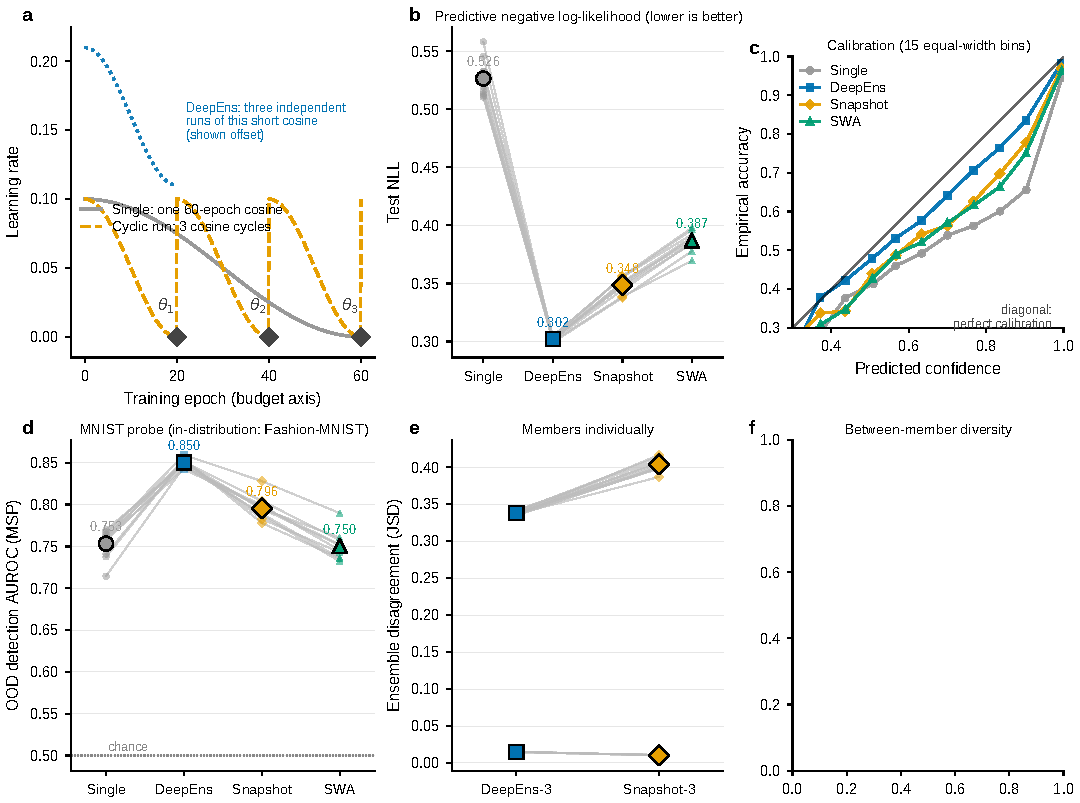
\includegraphics[width=\textwidth]{../figures/fig1_main.pdf}
\caption{\textbf{Budget-matched comparison of four uncertainty strategies.} \textbf{a}, Learning-rate schedules actually used in training, drawn on a shared budget axis: one 60-epoch cosine anneal (\single{}); a cyclic schedule of three cosine cycles whose cycle-end checkpoints $\theta_1$--$\theta_3$ (diamonds) form the \snapshot{} members and the \swa{} average; and the 20-epoch member schedule of \deepens{} (three independent runs of the schedule shown, offset for display). \textbf{b}, Test negative log-likelihood (NLL; lower is better). \textbf{c}, Reliability diagrams (15 equal-width confidence bins, mean over seeds); the diagonal marks perfect calibration. \textbf{d}, OOD-detection AUROC using the maximum-softmax score on an MNIST probe (in-distribution: Fashion-MNIST test); the dotted line marks chance. \textbf{e}, Mean test NLL of individual ensemble members. \textbf{f}, Between-member disagreement (mean pairwise Jensen--Shannon divergence, JSD). In \textbf{b}, \textbf{d}--\textbf{f}, thin grey lines connect the ten seed-level observations (small markers; conditions are additionally distinguished by marker shape as well as colour), large outlined markers show condition means, and the numbers above each condition give the mean ($n=10$ seeds; all observations shown; no exclusions). Ensemble size $k=3$ throughout.}
\label{fig:main}
\end{figure}

\subsection*{Every strategy improves NLL, with a strict ordering}

All three ensembling strategies improved the primary outcome, test NLL, over \single{} at matched budget (Table~\ref{tab:contrasts}, Fig.~\ref{fig:main}b): mean paired differences were $-0.2245$ (95\% CI $[-0.2360,-0.2130]$) for \deepens{}, $-0.1780$ ($[-0.1902,-0.1658]$) for \snapshot{} and $-0.1396$ ($[-0.1514,-0.1279]$) for \swa{}, each with exact sign-flip permutation $P=0.0020$ and Holm-adjusted $P=0.0098$ across the five pre-specified contrasts. The strategies were also strictly ordered: \deepens{} improved on \snapshot{} by $-0.0465$ ($[-0.0505,-0.0425]$) and \snapshot{} improved on \swa{} by $-0.0384$ ($[-0.0407,-0.0360]$), both with adjusted $P=0.0098$. The single long-trained network, by contrast, combined the highest accuracy trajectory per epoch with the worst predictive log-likelihood: its NLL of $0.5265 \pm 0.0159$ (mean $\pm$ s.d.) exceeded its own members' typical values despite accuracy of $0.8895 \pm 0.0015$, reflecting severe overconfidence rather than classification error.

The same ordering held on every secondary in-distribution metric (Table~\ref{tab:conditions}). Accuracy improved modestly but consistently (\deepens{} $+0.0070$, 95\% CI $[+0.0059,+0.0082]$; \snapshot{} $+0.0040$; \swa{} $+0.0031$ versus \single{}), the Brier score and expected calibration error (ECE) followed the NLL ordering, and the effect sizes were stable across seeds (all ten seeds favoured every strategy over \single{} for NLL).

\begin{table}[t]
\centering
\caption{\textbf{Test-set performance by condition} (mean $\pm$ s.d. over $n=10$ seeds; 10,000 Fashion-MNIST test images; OOD probe: 10,000 MNIST images). JSD and member NLL are defined only for the two ensemble conditions.}
\label{tab:conditions}
\small
\begin{tabular*}{\textwidth}{@{\extracolsep{\fill}} l cccc}
\toprule
Metric & \single{} & \deepens{} & \snapshot{} & \swa{} \\
\midrule
Test NLL (nats) & $0.5265 \pm 0.0159$ & $\mathbf{0.3020 \pm 0.0019}$ & $0.3485 \pm 0.0067$ & $0.3868 \pm 0.0085$ \\
Accuracy & $0.8895 \pm 0.0015$ & $\mathbf{0.8965 \pm 0.0012}$ & $0.8935 \pm 0.0015$ & $0.8926 \pm 0.0018$ \\
Brier score & $0.1796 \pm 0.0020$ & $\mathbf{0.1504 \pm 0.0011}$ & $0.1596 \pm 0.0024$ & $0.1646 \pm 0.0028$ \\
ECE (15 bins) & $0.0702 \pm 0.0021$ & $\mathbf{0.0236 \pm 0.0008}$ & $0.0444 \pm 0.0025$ & $0.0517 \pm 0.0025$ \\
AUROC (MSP score) & $0.7533 \pm 0.0172$ & $\mathbf{0.8502 \pm 0.0049}$ & $0.7956 \pm 0.0139$ & $0.7504 \pm 0.0168$ \\
AUROC (neg.\ entropy) & $0.7562 \pm 0.0172$ & $\mathbf{0.8657 \pm 0.0055}$ & $0.8059 \pm 0.0144$ & $0.7573 \pm 0.0171$ \\
\midrule
Member mean NLL & n/a & $0.3379 \pm 0.0022$ & $0.4039 \pm 0.0087$ & n/a \\
Disagreement JSD (nats) & n/a & $0.0150 \pm 0.0003$ & $0.0106 \pm 0.0003$ & n/a \\
\bottomrule
\end{tabular*}
\end{table}

\begin{table}[t]
\centering
\caption{\textbf{Pre-specified contrasts on the primary outcome (test NLL).} Mean paired difference $\Delta$ (condition A $-$ condition B), two-sided 95\% confidence interval, exact sign-flip permutation $P$ (all $2^{10}$ sign patterns), and Holm-adjusted $P$ across the five contrasts ($n=10$ seeds).}
\label{tab:contrasts}
\small
\begin{tabular*}{\textwidth}{@{\extracolsep{\fill}} l cccc}
\toprule
Contrast (A $-$ B) & $\Delta$ NLL & 95\% CI & $P_{\text{perm}}$ & $P_{\text{Holm}}$ \\
\midrule
\deepens{} $-$ \single{} & $-0.2245$ & $[-0.2360, -0.2130]$ & $0.0020$ & $0.0098$ \\
\snapshot{} $-$ \single{} & $-0.1780$ & $[-0.1902, -0.1658]$ & $0.0020$ & $0.0098$ \\
\swa{} $-$ \single{} & $-0.1396$ & $[-0.1514, -0.1279]$ & $0.0020$ & $0.0098$ \\
\deepens{} $-$ \snapshot{} & $-0.0465$ & $[-0.0505, -0.0425]$ & $0.0020$ & $0.0098$ \\
\snapshot{} $-$ \swa{} & $-0.0384$ & $[-0.0407, -0.0360]$ & $0.0020$ & $0.0098$ \\
\bottomrule
\end{tabular*}
\end{table}

\subsection*{Ensembling repairs calibration that longer training damages}

The reliability diagrams locate the NLL differences in the confidence scale (Fig.~\ref{fig:main}c and Supplementary Fig.~1). The single network's predictions clustered at high confidence with accuracy below that confidence: ECE was $0.0702 \pm 0.0021$, so that a typical predicted confidence of about $0.96$ was matched by roughly $0.89$ empirical accuracy. \deepens{} nearly restored calibration (ECE $0.0236 \pm 0.0008$, a $66\%$ reduction), \snapshot{} removed about a third of the error ($0.0444 \pm 0.0025$), and \swa{} about a quarter ($0.0517 \pm 0.0025$). The paired contrast for \deepens{} versus \single{} was $-0.0466$ ($95\%$ CI $[-0.0481,-0.0450]$). These calibration gains, rather than accuracy, carried most of the NLL improvement: \deepens{} removed $43\%$ of the single network's NLL excess.

\subsection*{OOD detection separates prediction averaging from weight averaging}

We next asked which budget allocations buy robustness, measured as the separation between in-distribution test images and MNIST images using the maximum-softmax (MSP) score\textsuperscript{7} (Fig.~\ref{fig:main}d and Supplementary Fig.~2 for the underlying score distributions). Here the strategies diverged qualitatively. \deepens{} improved AUROC by $+0.0969$ over \single{} ($95\%$ CI $[+0.0847,+0.1091]$, $P=0.0020$) and \snapshot{} by $+0.0423$ ($[+0.0291,+0.0555]$), whereas \swa{} showed \emph{no evidence} of improvement ($-0.0029$, $[-0.0166,+0.0109]$, $P=0.64$): the weight-averaged model detected the shift about as poorly as the single network it was built from. We note that the width of this interval (about $0.028$ AUROC units) bounds what this design can resolve; the claim is therefore one of absence of evidence, not of evidence of absence, and the same applies to the dense variant below ($-0.0075$, $[-0.0190,+0.0041]$). Because \snapshot{} and \swa{} combine the identical three checkpoints, this difference is attributable to the combination mechanism alone: averaging predictions transfers the ensemble's ability to disagree on shifted inputs into the score, while averaging weights collapses the members into one network whose confidence behaviour under shift is essentially that of the trajectory it came from. The same pattern held with the negative-entropy score ($\Delta$ AUROC for \swa{} versus \single{}: $+0.0011$), and the ranking of the other conditions was unchanged, indicating that the conclusion is not specific to the score function.

\subsection*{Why budget-split restarts win: member calibration and diversity}

The design also pins down why \deepens{} dominates \snapshot{} at matched budget (Fig.~\ref{fig:main}e,f); because the two ensembles share their first member, this contrast is carried by the second and third members, where the strategies differ in restarting versus continuing training. First, the individual members differed in calibration: the three independent 20-epoch restarts achieved a mean member NLL of $0.3379 \pm 0.0022$, whereas the second and third cyclic snapshots (taken after 40 and 60 cumulative epochs of continued training) were individually more overconfident ($0.4039 \pm 0.0087$ averaged over members), even though their member accuracy was nearly identical ($0.8912$ versus $0.8916$). Continued training on the same trajectory thus bought no member-level accuracy but cost member-level calibration. Second, the members were less diverse: the mean pairwise Jensen--Shannon divergence of member predictive distributions was $0.0150 \pm 0.0003$ nats for \deepens{} but only $0.0106 \pm 0.0003$ nats for \snapshot{}, a $30\%$ reduction in disagreement. Both quantities, member calibration and diversity, point in the direction that favours independent restarts; we note, however, that with $n=10$ seeds and $k=3$ members these measurements associate the mechanism with the outcome rather than establishing it causally.

Finally, we probed the robustness of the \swa{} conclusion, since our pre-registered \swa{} averages exactly three checkpoints (matching the \snapshot{} members), whereas standard practice averages many more. In a supplementary, explicitly exploratory analysis, we re-used the same trajectories and averaged every epoch-end checkpoint from epochs 21--60 (40 checkpoints). This \emph{dense} \swa{} improved NLL over \single{} ($-0.1598$, 95\% CI $[-0.1732,-0.1465]$; Supplementary Table~2) but still trailed the \snapshot{} ensemble ($+0.0182$, $[+0.0154,+0.0209]$) and, critically, still showed no evidence of improved OOD detection ($-0.0075$, $[-0.0190,+0.0041]$; Supplementary Fig.~3). Replacing 15-bin by 10-bin ECE, and the MSP by the negative-entropy score, left every pre-specified contrast's direction unchanged (Supplementary Table~1), so the reported ordering does not depend on these analysis choices.

% ─────────────────────────────── discussion ───────────────────────────────
\section*{Discussion}

At a fixed training budget, this experiment returns a clear ordering: splitting the budget across independent restarts (\deepens{}) produced the most accurate and best-calibrated uncertainty; a cyclic-schedule snapshot ensemble (\snapshot{}) captured most of the in-distribution benefit at one run's bookkeeping cost; and weight averaging (\swa{}) improved in-distribution metrics but, unlike either prediction-averaging strategy, showed no evidence of improving OOD detection. Because the four conditions shared data, architecture, optimizer, budget and pairing by seed, and because the \snapshot{} and \swa{} conditions shared the identical checkpoints, these differences are attributable to the allocation of the budget and the mechanism of combination rather than to tuning or trajectory noise.

The mechanism measurements suggest an interpretation in terms of where the two averaging operations act. Prediction averaging operates in function space: when members disagree, the mixture flattens the predictive distribution, which is exactly the behaviour that repairs overconfidence and that produces low-confidence predictions on shifted inputs. Weight averaging operates in parameter space: it selects a flatter, lower-loss point along the trajectory\textsuperscript{3,12}, which improves the network's fit--confidence trade-off in distribution, but it collapses the members' disagreement into a single confident model and thereby discards the epistemic signal that the shift detector consumes. Consistent with this reading, member-level analysis showed that continued-training snapshots are individually more overconfident than fresh restarts at equal accuracy, and less diverse from one another; the snapshot ensemble therefore starts from worse-calibrated, more correlated members than the budget-split ensemble even at the same budget. We emphasise that this account ties together associational measurements; a causal decomposition of the ensemble gain into member-quality and diversity components would require a dedicated design.

Our results are consistent with the literature that motivated the comparison (deep ensembles are strong but assumed expensive\textsuperscript{1,10}, snapshot ensembles are attractive because one run yields several models\textsuperscript{2}, and \swa{} improves accuracy and in-distribution calibration\textsuperscript{3,12}), but they quantify the trade-off under the constraint that matters in practice. The budget-matched framing reverses the usual cost accounting: a deep ensemble of three 20-epoch runs is not three times as expensive as one 60-epoch run; it \emph{is} the same budget spent differently. Under that accounting, the ``expensive'' strategy was uniformly best in this regime, the ``free'' strategies captured different fractions of its benefit, and the cheapest-to-deploy single-trajectory variant (\swa{}) bought no shift robustness. This complements benchmark studies that vary budgets across methods\textsuperscript{8,9} and echoes the observation that independent initialisation is the ingredient most responsible for ensemble gains\textsuperscript{10}: here that ingredient survives a three-fold reduction in per-member training.

For practitioners, the allocation rule we can support is as follows. At small scale and fixed compute, prefer independent restarts over longer training for calibrated uncertainty. If only a single trajectory is affordable, prefer its snapshot ensemble over its weight average when shift robustness matters. Treat \swa{} as an accuracy-and-fit tool rather than a shift detector, consistent with evidence that OOD failures often persist across training procedures\textsuperscript{7,13}. The rule is bounded by the scope of the evidence. Our study used one architecture family (a small multilayer perceptron without batch normalisation or dropout), one dataset family (Fashion-MNIST with an MNIST probe, both $28 \times 28$ grayscale), one budget ($B=60$ epochs) and one ensemble size ($k=3$). The \swa{} variant is checkpoint-matched to the snapshot ensemble by design, and although a dense 40-checkpoint average did not change the qualitative conclusion, other \swa{} schedules might. The OOD probe is a single dataset-shift pair rather than a spectrum of shifts. Finally, no post-hoc recalibration (for example, temperature scaling on a held-out set\textsuperscript{5}) was applied, so the comparison reflects uncalibrated deployment. Extending the design along these axes---larger networks, harder shifts, budget and ensemble-size scaling, and stacked post-hoc calibration---is the natural next step, and the paired, seed-replicated template used here is directly reusable for it.

% ─────────────────────────────── methods ───────────────────────────────
\section*{Methods}

\subsection*{Datasets and splits}
Fashion-MNIST\textsuperscript{18} (60,000 training and 10,000 test images, $28 \times 28$ grayscale, ten classes) served as the in-distribution task, and the MNIST\textsuperscript{19} test set (10,000 images) as the OOD probe. The training set was split once, with a fixed split seed, into 54,000 training and 6,000 validation images; class counts were exactly balanced (6,000 per class in the full training set). Images were scaled to $[0,1]$ and standardised with the mean and standard deviation of the training split. The validation split was used only for monitoring and learning curves (Supplementary Fig.~4); no early stopping, hyperparameter selection or model selection was performed on validation or test data. The test set was evaluated exactly once per condition per seed, after all training was complete.

\subsection*{Architecture and training}
All networks were multilayer perceptrons with layers 784--128--64--10 and ReLU activations ($\approx$110k parameters), without dropout or batch normalisation. Training used mini-batch SGD with batch size 256 (211 steps per epoch on 54,000 images), momentum 0.9 and weight decay $10^{-4}$ (coupled). Learning rates followed per-step cosine schedules from $\eta_{\max}=0.1$ to $0$: a single 60-epoch anneal for \single{}, three 20-epoch cycles for the cyclic run, and one 20-epoch anneal per \deepens{} member. Initialisation used PyTorch's default Kaiming-uniform scheme; data order per run was generated from a dedicated seeded generator. Hyperparameters were fixed from common practice before any test-set evaluation; a pilot confirmed training stability (monotonically decreasing training loss, no divergence) using training and validation losses only. Training the full experiment took approximately 160 epochs per seed (ten seeds) on two CPU cores, about 13 minutes per seed; the supplementary dense-\swa{} pass re-ran the cyclic trajectories with per-epoch checkpointing (about 5 minutes per seed).

\subsection*{Budget-matched conditions}
Within each seed $s$, run seeds were derived deterministically from a base value ($10{,}000 + 100s$). \single{} used seed $b$ and trained 60 epochs. The cyclic run used the same seed $b$, trained 60 epochs in three cosine cycles, and stored deep copies of the network at each cycle end ($\theta_1$, $\theta_2$, $\theta_3$). Because a cosine cycle of 20 epochs under seed $b$ is a complete anneal, $\theta_1$ is bit-identical to a fresh 20-epoch run with seed $b$; this equality was verified programmatically for seed 0 (all state tensors compared exactly) and exploited so that $\theta_1$ serves as the first member of both ensembles. The second and third \deepens{} members were fresh 20-epoch runs with distinct seeds. \snapshot{} predicts with the mean of the softmax outputs of $\theta_1,\theta_2,\theta_3$; \swa{} predicts with the network whose weights are the uniform average of the same three state dicts. The supplementary \emph{SWA-dense} condition (exploratory, not pre-registered) re-used the cyclic trajectories and averaged all epoch-end checkpoints from epochs 21--60.

\subsection*{Evaluation metrics}
All metrics were computed on the full test set (and, for OOD, the full MNIST probe) with probabilities evaluated in float64. NLL is the mean negative log-probability of the true class under the (ensemble-mean) predictive distribution. Accuracy is the fraction of argmax-correct predictions. The Brier score is the mean over samples of the summed squared error between the predictive distribution and the one-hot label. ECE uses 15 equal-width bins over maximum predicted probability\textsuperscript{6} (sensitivity: 10 bins). OOD detection uses the AUROC of the maximum-softmax score\textsuperscript{7} with in-distribution samples as positives (sensitivity: the negative-entropy score). Ensemble disagreement is the mean over test samples and member pairs of the Jensen--Shannon divergence between the two member predictive distributions (natural logarithm). Ensemble predictive distributions are the arithmetic mean of member softmax outputs.

\subsection*{Statistical analysis}
The analysis plan (including the contrast set, the primary outcome and the multiplicity strategy) was written and stored before any test-set evaluation; the only amendment (increasing replications from five to ten seeds) was made after a timing pilot, before any outcome was observed, and cannot bias paired contrasts. The independent experimental unit is the seed; each seed contributes one value per condition per metric, and all contrasts are within-seed paired differences. We report mean differences with two-sided 95\% $t$-intervals ($n-1=9$ degrees of freedom), exact two-sided sign-flip permutation $P$ values enumerating all $2^{10}$ sign patterns, and Holm--Bonferroni adjustment across the five pre-specified contrasts applied to the primary outcome (NLL); secondary metrics are reported as uncorrected effect estimates. Sensitivity analyses (10-bin ECE, entropy-based AUROC score, dense \swa{}) were specified in advance or, for dense \swa{}, labelled exploratory. No data were excluded; no condition, seed or sample was dropped at any stage.

\subsection*{Reproducibility}
Experiments used PyTorch 2.14.0 (CPU), NumPy 2.1.3, SciPy 1.14.1 and scikit-learn 1.5.2 on Python 3.12.14 (two CPU cores, no GPU). Every training run is deterministic given its seed; re-running seed 0 reproduced all 24 recorded metrics exactly (bit-level verification). The complete study consumed 2,200 training epochs in total: 1,600 epochs for the pre-registered experiment (160 per seed, ten seeds; about 13 minutes of single-machine CPU time) and 600 epochs for the supplementary dense-\swa{} pass (about 5 minutes). Training, analysis and figure scripts, the raw per-seed metric records, figure source data and the analysis plan are released with the manuscript.

% ─────────────────────────────── references ───────────────────────────────
\begin{thebibliography}{19}
\small

\bibitem{lakshminarayanan2017} Lakshminarayanan, B., Pritzel, A. \& Blundell, C. Simple and scalable predictive uncertainty estimation using deep ensembles. \emph{Adv. Neural Inf. Process. Syst.} \textbf{30} (2017).

\bibitem{huang2017} Huang, G., Li, Y., Pleiss, G., Liu, Z., Hopcroft, J. E. \& Weinberger, K. Q. Snapshot ensembles: train 1, get M for free. \emph{Int. Conf. Learn. Represent.} (2017).

\bibitem{izmailov2018} Izmailov, P., Podoprikhin, D., Garipov, T., Vetrov, D. \& Wilson, A. G. Averaging weights leads to wider optima and better generalization. \emph{Conf. Uncertain. Artif. Intell.} (2018).

\bibitem{loshchilov2017} Loshchilov, I. \& Hutter, F. SGDR: stochastic gradient descent with warm restarts. \emph{Int. Conf. Learn. Represent.} (2017).

\bibitem{guo2017} Guo, C., Pleiss, G., Sun, Y. \& Weinberger, K. Q. On calibration of modern neural networks. \emph{Int. Conf. Mach. Learn.} (2017).

\bibitem{naeini2015} Naeini, M. P., Cooper, G. \& Hauskrecht, M. Obtaining well calibrated probabilities using Bayesian binning into quantiles. \emph{AAAI Conf. Artif. Intell.} (2015).

\bibitem{hendrycks2017} Hendrycks, D. \& Gimpel, K. A baseline for detecting misclassified and out-of-distribution examples in neural networks. \emph{Int. Conf. Learn. Represent.} (2017).

\bibitem{ashukha2020} Ashukha, A. et al. Pitfalls of in-domain uncertainty estimation and ensembling. \emph{Int. Conf. Learn. Represent.} (2020).

\bibitem{ovadia2019} Ovadia, Y. et al. Can you trust your model's uncertainty? Evaluating predictive uncertainty under dataset shift. \emph{Adv. Neural Inf. Process. Syst.} \textbf{32} (2019).

\bibitem{fort2019} Fort, S., Hu, H. \& Lakshminarayanan, B. Deep ensembles: a loss landscape perspective. Preprint at \url{https://arxiv.org/abs/1912.02757} (2019).

\bibitem{gal2016} Gal, Y. \& Ghahramani, Z. Dropout as a Bayesian approximation: representing model uncertainty in deep learning. \emph{Int. Conf. Mach. Learn.} (2016).

\bibitem{wilson2020} Wilson, A. G. \& Izmailov, P. Bayesian deep learning and a probabilistic perspective of generalization. \emph{Adv. Neural Inf. Process. Syst.} \textbf{33} (2020).

\bibitem{maddox2019} Maddox, W. J., Izmailov, P., Garipov, T., Vetrov, D. P. \& Wilson, A. G. A simple baseline for Bayesian uncertainty in deep learning. \emph{Adv. Neural Inf. Process. Syst.} \textbf{32} (2019).

\bibitem{nguyen2015} Nguyen, A., Yosinski, J. \& Clune, J. Deep neural networks are easily fooled: high confidence predictions for unrecognizable images. \emph{IEEE Conf. Comput. Vis. Pattern Recognit.} (2015).

\bibitem{welling2011} Welling, M. \& Teh, Y. W. Bayesian learning via stochastic gradient Langevin dynamics. \emph{Int. Conf. Mach. Learn.} (2011).

\bibitem{abdar2021} Abdar, M. et al. A review of uncertainty quantification in deep learning: techniques, applications and challenges. \emph{Inf. Fusion} \textbf{76}, 243--297 (2021).

\bibitem{xiao2017} Xiao, H., Rasul, K. \& Vollgraf, R. Fashion-MNIST: a novel image dataset for benchmarking machine learning algorithms. Preprint at \url{https://arxiv.org/abs/1708.07747} (2017).

\bibitem{lecun1998} LeCun, Y., Bottou, L., Bengio, Y. \& Haffner, P. Gradient-based learning applied to document recognition. \emph{Proc. IEEE} \textbf{86}, 2278--2324 (1998).

\end{thebibliography}

% ─────────────────────── supplementary information ───────────────────────
\section*{Supplementary Information}

\begin{figure}[htbp]
\centering
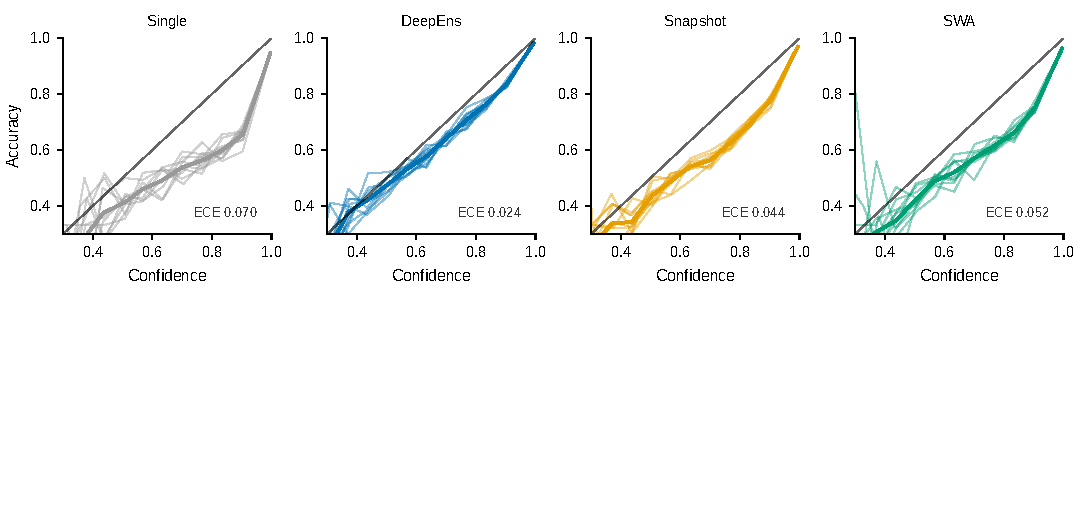
\includegraphics[width=\textwidth]{../figures/suppl_fig1_reliability.pdf}
\caption{\textbf{Supplementary Figure 1 | Reliability diagrams per condition.} Thin lines show the ten individual seeds; the bold line shows the seed-mean reliability curve (15 equal-width bins). ECE (mean over seeds) is annotated in each panel. The single network's curve lies furthest below the diagonal at high confidence; \deepens{} lies closest to it.}
\label{fig:supp1}
\end{figure}

\begin{figure}[htbp]
\centering
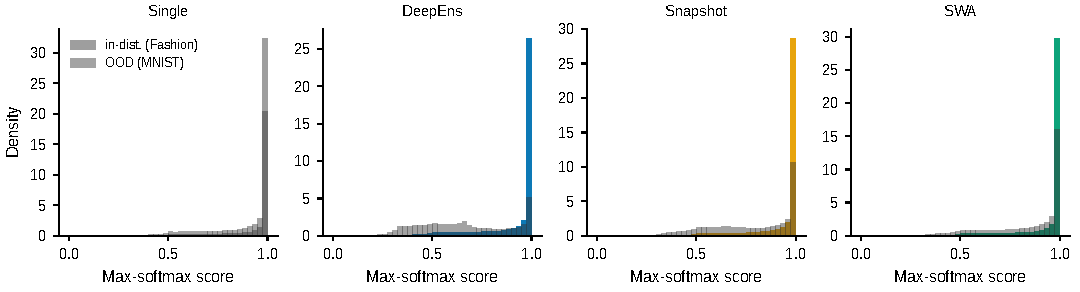
\includegraphics[width=\textwidth]{../figures/suppl_fig2_msp_hist.pdf}
\caption{\textbf{Supplementary Figure 2 | Maximum-softmax score distributions underlying the OOD analysis.} Mean score density over the ten seeds, in-distribution (Fashion-MNIST test; coloured) versus OOD probe (MNIST; grey). The two prediction-averaging strategies shift OOD scores leftward (lower confidence on shifted inputs) substantially more than \swa{} does, which is the direct visual counterpart of the AUROC result in Fig.~1d.}
\label{fig:supp2}
\end{figure}

\begin{figure}[htbp]
\centering
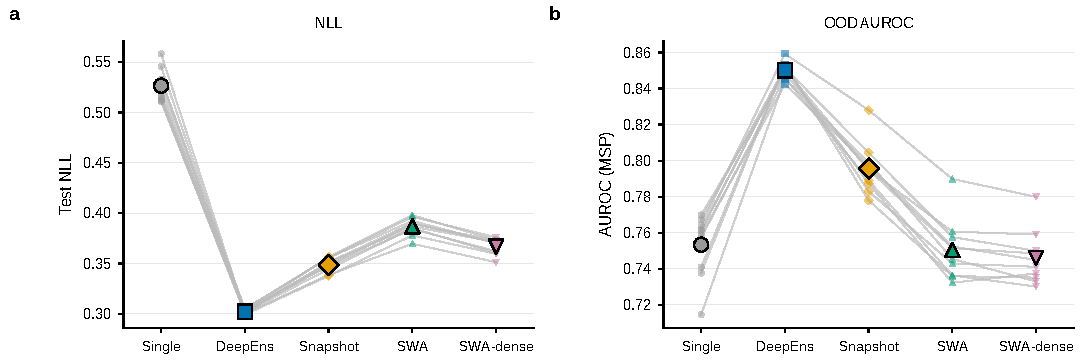
\includegraphics[width=0.72\textwidth]{../figures/suppl_fig3_swa_dense.pdf}
\caption{\textbf{Supplementary Figure 3 | Exploratory dense weight-averaging variant.} \textbf{a}, Test NLL and \textbf{b}, OOD AUROC for the pre-registered conditions plus the exploratory \emph{SWA-dense} variant (uniform average of all epoch-end checkpoints from epochs 21--60 of the same cyclic trajectories). Dense averaging improves the in-distribution metrics over \swa{} but does not close the gap to the snapshot ensemble and leaves OOD detection unchanged from \single{}.}
\label{fig:supp3}
\end{figure}

\begin{figure}[htbp]
\centering
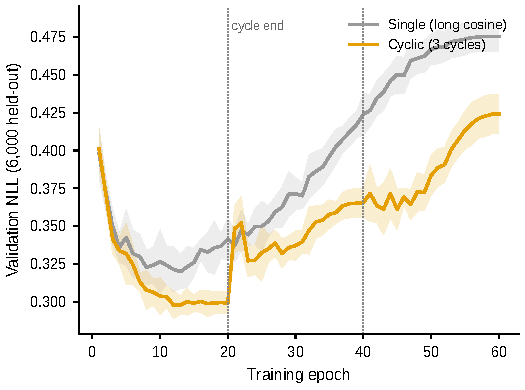
\includegraphics[width=0.55\textwidth]{../figures/suppl_fig4_curves.pdf}
\caption{\textbf{Supplementary Figure 4 | Validation learning curves of the two training trajectories.} Mean $\pm$ s.d. of validation NLL (6,000 held-out images) over the ten seeds for the single 60-epoch cosine anneal and the cyclic three-cycle run. Dotted vertical lines mark cycle boundaries (epochs 20 and 40).}
\label{fig:supp4}
\end{figure}

\begin{table}[htbp]
\centering
\caption{\textbf{Supplementary Table 1 | Pre-specified contrasts on secondary metrics} (mean paired difference $\Delta$, 95\% CI, exact permutation $P$; $n=10$ seeds; uncorrected, descriptive).}
\label{tab:supp1}
\footnotesize
\begin{tabular*}{\textwidth}{@{\extracolsep{\fill}} l l ccc}
\toprule
Metric & Contrast (A $-$ B) & $\Delta$ & 95\% CI & $P_{\text{perm}}$ \\
\midrule
Accuracy & \deepens{} $-$ \single{} & $+0.0070$ & $[+0.0059, +0.0082]$ & $0.0020$ \\
 & \snapshot{} $-$ \single{} & $+0.0040$ & $[+0.0025, +0.0055]$ & $0.0020$ \\
 & \swa{} $-$ \single{} & $+0.0031$ & $[+0.0014, +0.0048]$ & $0.0020$ \\
 & \deepens{} $-$ \snapshot{} & $+0.0030$ & $[+0.0019, +0.0041]$ & $0.0039$ \\
 & \snapshot{} $-$ \swa{} & $+0.0009$ & $[+0.0004, +0.0013]$ & $0.0078$ \\
\midrule
Brier score & \deepens{} $-$ \single{} & $-0.0292$ & $[-0.0311, -0.0274]$ & $0.0020$ \\
 & \snapshot{} $-$ \single{} & $-0.0200$ & $[-0.0224, -0.0176]$ & $0.0020$ \\
 & \swa{} $-$ \single{} & $-0.0150$ & $[-0.0176, -0.0125]$ & $0.0020$ \\
 & \deepens{} $-$ \snapshot{} & $-0.0093$ & $[-0.0107, -0.0078]$ & $0.0020$ \\
 & \snapshot{} $-$ \swa{} & $-0.0050$ & $[-0.0053, -0.0046]$ & $0.0020$ \\
\midrule
ECE (15 bins) & \deepens{} $-$ \single{} & $-0.0466$ & $[-0.0481, -0.0450]$ & $0.0020$ \\
 & \snapshot{} $-$ \single{} & $-0.0258$ & $[-0.0275, -0.0241]$ & $0.0020$ \\
 & \swa{} $-$ \single{} & $-0.0184$ & $[-0.0202, -0.0167]$ & $0.0020$ \\
 & \deepens{} $-$ \snapshot{} & $-0.0208$ & $[-0.0224, -0.0191]$ & $0.0020$ \\
 & \snapshot{} $-$ \swa{} & $-0.0073$ & $[-0.0080, -0.0067]$ & $0.0020$ \\
\midrule
AUROC (MSP) & \deepens{} $-$ \single{} & $+0.0969$ & $[+0.0847, +0.1091]$ & $0.0020$ \\
 & \snapshot{} $-$ \single{} & $+0.0423$ & $[+0.0291, +0.0555]$ & $0.0020$ \\
 & \swa{} $-$ \single{} & $-0.0029$ & $[-0.0166, +0.0109]$ & $0.6406$ \\
 & \deepens{} $-$ \snapshot{} & $+0.0546$ & $[+0.0452, +0.0640]$ & $0.0020$ \\
 & \snapshot{} $-$ \swa{} & $+0.0452$ & $[+0.0402, +0.0501]$ & $0.0020$ \\
\midrule
AUROC (neg.\ entropy) & \deepens{} $-$ \single{} & $+0.1095$ & $[+0.0970, +0.1220]$ & $0.0020$ \\
 & \snapshot{} $-$ \single{} & $+0.0497$ & $[+0.0361, +0.0633]$ & $0.0020$ \\
 & \swa{} $-$ \single{} & $+0.0011$ & $[-0.0129, +0.0152]$ & $0.8672$ \\
 & \deepens{} $-$ \snapshot{} & $+0.0598$ & $[+0.0499, +0.0697]$ & $0.0020$ \\
 & \snapshot{} $-$ \swa{} & $+0.0485$ & $[+0.0434, +0.0536]$ & $0.0020$ \\
\bottomrule
\end{tabular*}
\end{table}

\begin{table}[htbp]
\centering
\caption{\textbf{Supplementary Table 2 | Exploratory dense weight-averaging variant (\emph{SWA-dense})}, uniform average of all epoch-end checkpoints from epochs 21--60 of the same cyclic trajectories ($n=10$ seeds; exploratory, uncorrected).}
\label{tab:supp2}
\small
\begin{tabular*}{\textwidth}{@{\extracolsep{\fill}} l ccc}
\toprule
Metric & \emph{SWA-dense} (mean $\pm$ s.d.) & vs \single{} ($\Delta$, 95\% CI) & vs \snapshot{} ($\Delta$, 95\% CI) \\
\midrule
Test NLL & $0.3666 \pm 0.0079$ & $-0.1598\ [-0.1732, -0.1465]$ & $+0.0182\ [+0.0154, +0.0209]$ \\
ECE (15 bins) & $0.0460 \pm 0.0023$ & $-0.0242\ [-0.0260, -0.0224]$ & $+0.0016\ [+0.0003, +0.0029]$ \\
AUROC (MSP) & $0.7458 \pm 0.0149$ & $-0.0075\ [-0.0190, +0.0041]$ & $-0.0498\ [-0.0561, -0.0435]$ \\
\bottomrule
\end{tabular*}
\end{table}

\section*{Data and code availability}
All training, analysis and figure scripts (Python), the raw per-seed metric records (JSONL), the aggregated analysis outputs (JSON/CSV), the figure source data (one CSV per panel) and the pre-registered analysis plan accompany this manuscript; the datasets used are publicly available (Fashion-MNIST and MNIST). Author names, affiliations and the choice of licence are pending author confirmation.

\end{document}
